\documentclass[a4paper, 12pt,oneside]{article}
\usepackage{graphicx} % Required for inserting images
\usepackage[top=2.5cm, bottom=2cm, left=2cm, right=2cm]{geometry}
\usepackage[T1]{fontenc}
\usepackage[utf8]{inputenc}
\usepackage[colorlinks,bookmarks=false,linkcolor=black,urlcolor=blue, citecolor=black]{hyperref}
\usepackage{units}
\usepackage{verbatim}
\usepackage{verbdef}% http://ctan.org/pkg/verbdef
\usepackage{amsmath}
\usepackage{amssymb}
\usepackage{wrapfig}
\usepackage{subcaption}
\usepackage{caption}
\usepackage{float}
\usepackage[export]{adjustbox}
\usepackage{upgreek}
\usepackage{hyperref}
%Pour changer la taille des titres de section et subsection. Ajoutez manuellement les autres styles si besoin.
\makeatletter
\renewcommand{\section}{\@startsection {section}{1}{\z@}%
             {-3.5ex \@plus -1ex \@minus -.2ex}%
             {2.3ex \@plus.2ex}%
             {\normalfont\normalsize\bfseries}}
\makeatother

\makeatletter
\renewcommand{\subsection}{\@startsection {subsection}{1}{\z@}%
             {-3.5ex \@plus -1ex \@minus -.2ex}%
             {2.3ex \@plus.2ex}%
             {\normalfont\normalsize\bfseries}}
\makeatother

\graphicspath{{Images/}}
\graphicspath{{Graphes/}}
\graphicspath{{Graphes/comparaison/}}
\graphicspath{{Graphes/critique/}}
\graphicspath{{Graphes/Gain/}}
\graphicspath{{Graphes/Phase/}}
\graphicspath{{Graphes/souscritique/}}
\graphicspath{{Graphes/surcritique/}}


\title{Travaux Pratiques n°G3: Circuits RCL}
\author{Groupe n°22: Armand Le Douarec}
\date{21 Septembre 2024}

\begin{document}

\maketitle

\section{Introduction}

Les oscillations harmoniques, qu'elles soient libres ou forcées, sont des phénomènes observés dans divers domaines de la physique. Elles se manifestent tant dans l'aéronautique [\ref{ref1}] que dans la construction de ponts. L'étude de ces phénomènes, devenue essentielle, se retrouve ici dans le contexte des circuits RCL. L'effondrement du pont de Tacoma [\ref{Tacoma}] illustre parfaitement l'importance de ce sujet. L'analyse de ces circuits permet ainsi d'aborder des problèmes mécaniques variés en simulant les paramètres spécifiques de chaque situation.\\
Différents aspects de ces oscillations seront abordés, d'abord les oscillations libres puis les oscillations forcées et enfin une légère comparaison des filtres basiques constructibles à partir de ce circuit.
\section{Théorie}
Un circuit RCL est constitué de trois dipôles, une résistance $R$, une capacité $C$ et enfin une inductance $L$. Le montage est celui illustré sur la Fig.(\ref{Montage}) avec $U_{in}$ la tension du signal d'entrée et $U_{out}$ la tension de sortie. Pour construire l'équation qui caractérise le circuit RCL donné, les équations tension-courant de la résistance, de la capacité et de l'inductance sont nécessaires. Elles sont respectivement:
\begin{equation}
    U_R=RI_R\qquad CU_C=\int I_C \,dt \qquad U_L=-L\frac{dI_L}{dt}
\end{equation}

\begin{wrapfigure}{l}{0.4\textwidth}
\vspace{-1.1cm}
\includegraphics[width=1\linewidth]{Images/Circuit}
\captionsetup{justification=centering}
\caption{Représentation du circuit RCL étudié}
\label{fig:wrapfig}
\label{Montage}
\end{wrapfigure}

 A partir de ces équations ainsi que des lois de Kirchhoff, s'établit l'équation attendue qu'est l'équation différentielle du second ordre suivante:

\begin{equation}
    \ddot{U}_{out}+\frac{\dot{U}_{out}}{RC}+\frac{U_{out}}{LC} = \frac{U_{in}}{LC}
    \label{equation_de_base}
\end{equation}

Pour la suite des calculs, il est judicieux d'effectuer les simplifications suivantes pour mieux décrire le comportement du circuit. Ce sont la pulsation harmonique $w_0 = \sqrt{1/(LC)}$ en s$^{-1}$,  le coefficient d'amortissement $\lambda = 1/(2RC)$ en s$^{-1}$ et enfin la perturbation sinusoïdale $p\sin(\Omega t) = U_{in}$ d'amplitude $p$ et de fréquence $\Omega$. L'équation (\ref{equation_de_base}) devient alors:

\begin{equation}
    (\ref{equation_de_base}) \Rightarrow U_{out}+2\lambda\dot{U}_{out}+w_0^2\ddot{U}_{out}=p\sin(\Omega t)
    \label{final_eq}
\end{equation}

Les solutions de l'équation dépendent à présent des coefficients $w_0$ et $\lambda$. On remarque une analogie avec l'oscillateur mécanique qui est facilement simulable à l'aide de ce circuit.
\subsection*{Solutions}

Les solutions de l'équation (\ref{final_eq}) sont trois, et se différencient par les valeurs des paramètres $\lambda$ et $w_0$. Elles sont la somme de deux expressions décrivant le régime permanent et le régime transitoire. Elles sont données par:
\begin{equation}
\left\{\begin{array}{ll}
U_{out}(t) = A(\Omega)\sin(\Omega t-\psi (\Omega))+Ce^{-\lambda t}\cos(wt-\phi) & ,\lambda^2 < w_0^2 \ ,\text{(sous-critique)}\\
U_{out}(t) = A(\Omega)\sin(\Omega t-\psi (\Omega))+e^{-\lambda t}(C_1+C_2t)) & ,\lambda^2=w_0^2 \ ,\text{(critique)}\\
U_{out}(t) = \underbrace{A(\Omega)\sin(\Omega t-\psi (\Omega))}_{\text{régime permanent}}+\underbrace{e^{-\lambda t}(C_1 e^{w t}+C_2 e^{-w t})}_{\text{régime transitoire}} & , \lambda^2 > w_0^2 \ ,\text{(surcritique)}
\end{array}
\right.
\label{eq_boss}
\end{equation}

où les constantes $C,\, C_1,\, C_2\, \text{et } \phi$ sont déterminées par les conditions initiales et $w^2 = w_0^2 -\lambda^2$. Les fonctions de gain $A(\Omega) (\equiv U_{out}/U_{in})$ et de phase $\psi(\Omega)$ sont données par:

\begin{equation}
A(\Omega)= \frac{p}{\sqrt{(w_0^2-\Omega^2)^2+(2\lambda\Omega)^2}} \qquad \psi(\Omega)=\arctan\left(\frac{2\lambda\Omega}{w_0^2-\Omega^2}\right)
\end{equation}
\vspace{-0.4cm}
\subsection*{Oscillations libres}

Dans le cas d'oscillations libres, $p=0$. Par conséquent, la solution ne comprend plus que l'expression du régime transitoire. Une impulsion doit être donnée au circuit pour analyser son retour au régime stable. Le comportement du circuit est alors semblable à celui d'un oscillateur mécanique en mouvement soumis à une force de frottement au système (ici analogue à $\lambda$).\\
Les résistances internes de l'inductance $R_L$ et du générateur de fonction $R_G$ non négligeables doivent être considérées dans l'expression du coefficient d'amortissement. En série, la résistance interne résultante est $R_{in}=R_G+R_L$. Le coefficient d'amortissement devient alors:
\vspace{-0.1cm}
\begin{equation}
    \lambda^{'} = \lambda+R_{in}/(2L)
    \label{eq'}
    \vspace{-0.1cm}
\end{equation}
Dans le cas d'oscillations forcées, la résistance interne du générateur est prise en compte par le logiciel. Par conséquent, $R_{in} = R_L$ pour les oscillations forcées.
\vspace{-0.2cm}

\subsection*{Oscillations forcées}
\vspace{-0.1cm}
Dans ce type d'oscillation le régime permanent importe et une nouvelle donnée fondamentale 
 apparaît, $\Omega_r$, la pulsation résonante représentant la fréquence à laquelle le gain du système est maximal. L'expression de cette fréquence est donnée par $\Omega_r = \sqrt{w_0^2-2\lambda^2}$ (peut être calculée comme maximum de $A(\Omega)$). Pour décrir la finesse de la résonance, il est judicieux d'utiliser le facteur de qualité de la résonance $Q$ donné par l'expression $Q = \frac{\Delta\Omega}{\Omega_r}$; ainsi que la largeur de raie $\Delta\Omega$ donnée par $\Delta\Omega = \Omega_1-\Omega_2 = \frac{2\lambda\Omega}{\Omega_r}$ où $\Omega_1$ et $\Omega_2$ sont les fréquences telles que le gain A évalué en ces dernières vaut $A_{max}/\sqrt{2}$. A partir d'un diagramme de Bode du gain $G(\Omega)$ et de la phase $\phi(\Omega)$ du signal obtenu, le pic $G_{max}$ et la finesse de résonance $\Delta\Omega$ ainsi que le coefficient d'amortissement expérimental $\lambda_{exp}$ peuvent être obtenus pour en déduire la nature du filtre, notamment grâce à l'équation:
\vspace{-0.1cm}
\begin{equation}
\lambda_{exp}=\Omega_r \sqrt{\frac{1}{2}\left(\sqrt{\frac{G_{max}^2}{G_{max}^2-1}}-1\right)}\qquad \text{avec $G_{max} = G(\Omega_r)$}
\label{eq_lambda}
\end{equation}
 \vspace{-0.5cm}
\section{Résultats}
Dans cette étude, les valeurs constantes des composantes du système étaient $L = 0.05$ H,\\
$ C = 0.01 \,\upmu$F et les résistances internes du générateur et de l'inductance sont $R_G = (50.0 \pm 0.1)\,\Omega$ et $R_L = (207.0 \pm 0.3)\,\Omega$ mesurées à l'aide du multimètre.
\subsection*{Oscillations libres}

Dans l'étude des oscillations libres, différentes valeurs de la résistance ont été testées pour chaque régime transitoire. Le générateur de fonction produisait un signal carré de fréquence de l'ordre de $ f \simeq 100$ Hz et un oscilloscope digital a permis d'effectuer les mesures. La résistance critique a été trouvée en $R_{cr} = 1240\,\Omega$. La résistance interne à prendre en compte est ici $R_{in} = R_G+R_L = (257.0\pm0.4)\,\Omega$. De plus, la tension du signal mesurée est relevée à une période $\Delta t = 0.4 [\upmu$s].\\

\begin{figure}[h]
\vspace{-0.85cm}
\centering  % Centrer tout l'ensemble
\begin{subfigure}{0.45\textwidth}  % Réduire la taille pour s'assurer qu'elles tiennent côte à côte
    \centering  % Centrer cette sous-figure
    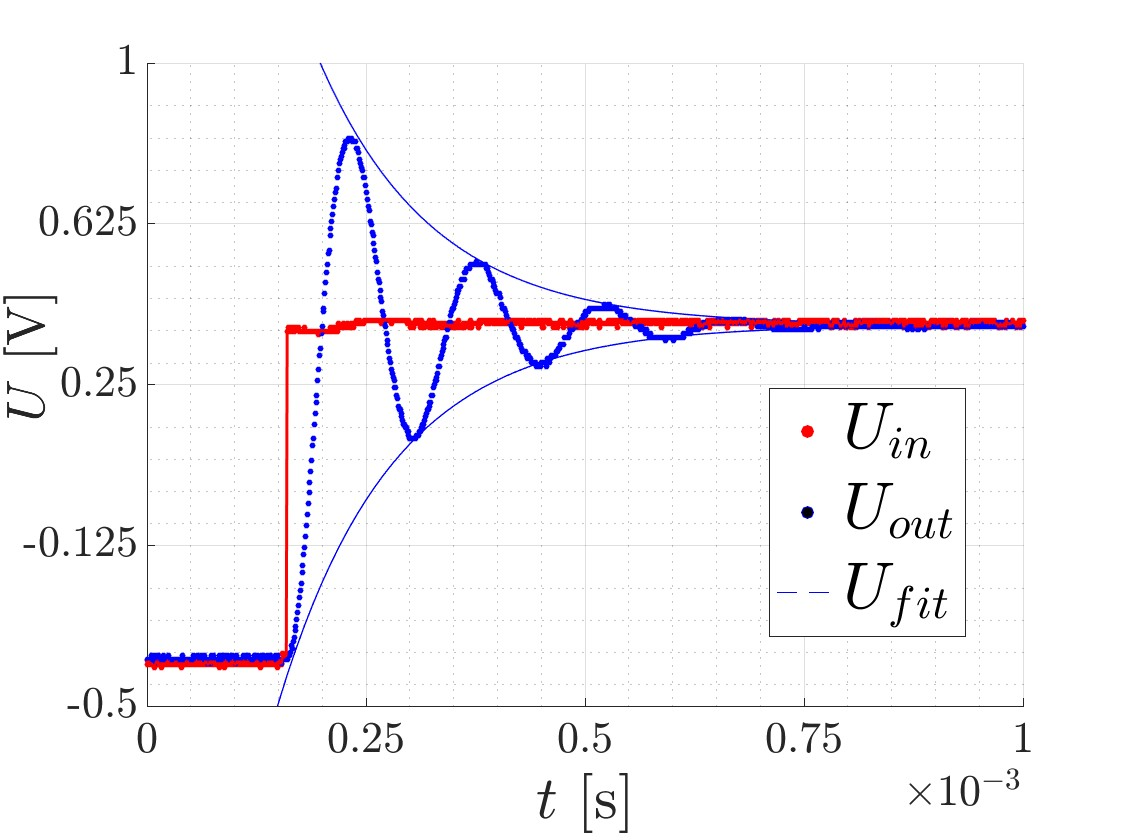
\includegraphics[width=1.15\linewidth, height=5.3cm]{Graphes/souscritique/sous_critique_10}
    \captionsetup{justification=centering}
    \caption{$R =(10\pm 0.1)$ k$\Omega$}
    \label{fig2a}
\end{subfigure}
\begin{subfigure}{0.45\textwidth}  % Réduire également ici
    \centering  % Centrer cette sous-figure
    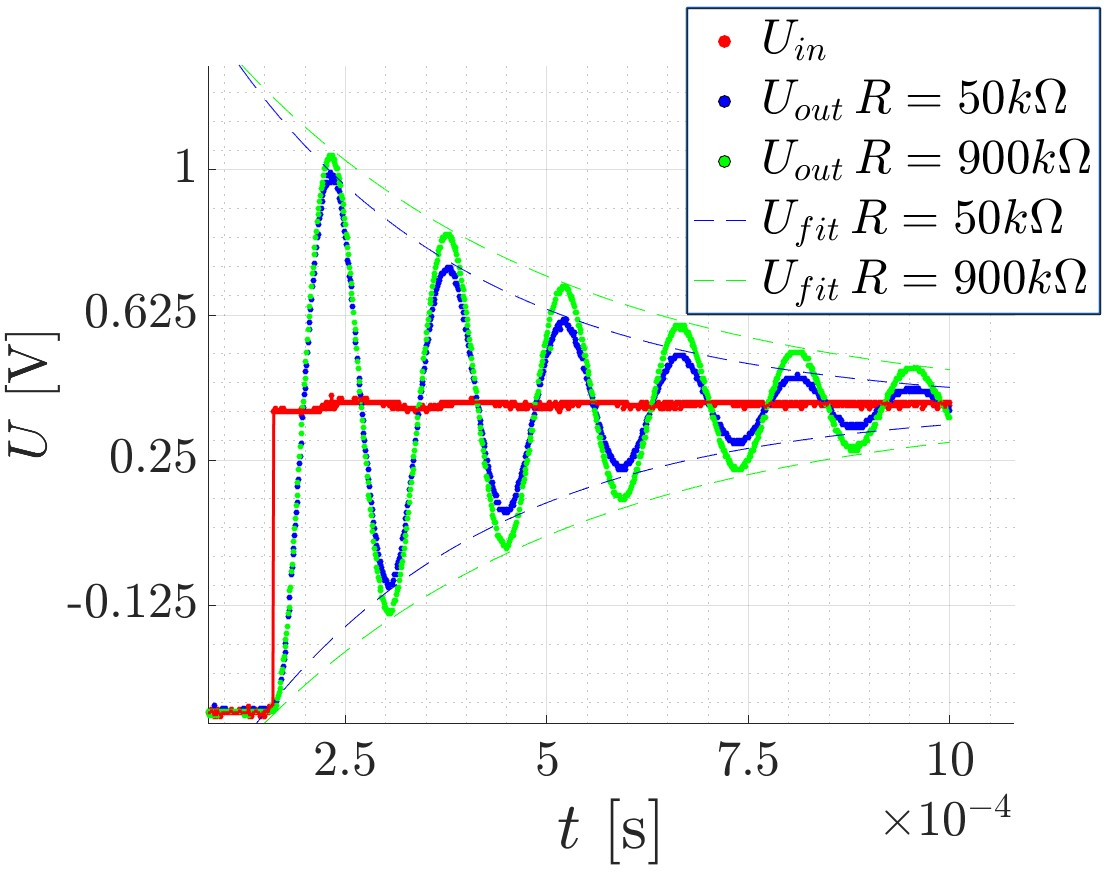
\includegraphics[width=1\linewidth, height = 5.3cm]{Graphes/souscritique/sous_critique_50k_90k}
    \captionsetup{justification=centering}
    \caption{$R =(50\pm 0.5)$ k$\Omega, $ et $R =(900\pm 9) $ k$\Omega$}
    \label{fig2b}
\end{subfigure}
\captionsetup{justification=centering}
\vspace{-0.2cm}
\caption{Graphes $U$[V] en fonction de $t$[s] pour différentes valeurs de $R$ en régime souscritique}
\label{fig2}
\vspace{-0.5cm}
\end{figure}
Pour le régime sous-critique, $ R> R_{cr}$, les Fig.(\ref{fig2a}) et Fig.(\ref{fig2b}) montrent la réponse du signal pour des résistances allant de $10$ k$\Omega$ à $900$ k$\Omega$. De plus, un fit exponentiel a été effectué pour analyser l'enveloppe de chaque oscillation en régime sous-critique, permettant ainsi de trouver expérimentalement $\lambda_{exp}$ grâce au coefficient du fit. Les coefficient seront notés dans le Tab.(\ref{table1}).\\
Pour le régime critique, $ R = R_{cr}$, la Fig.(\ref{fig3}). présente la réponse du signal avec un fit exponentiel pour mesurer $\lambda_{exp}(=w_0)=40$ [ms$^{-1}$].\\
Pour le régime surcritique, la Fig.(\ref{fig4}) la réponse du signal pour des résistances allant de $100\,\Omega$ à $800\,\Omega$.\\
\begin{wrapfigure}{h}{0.4\textwidth}
\vspace{-1.2cm}
\raggedright
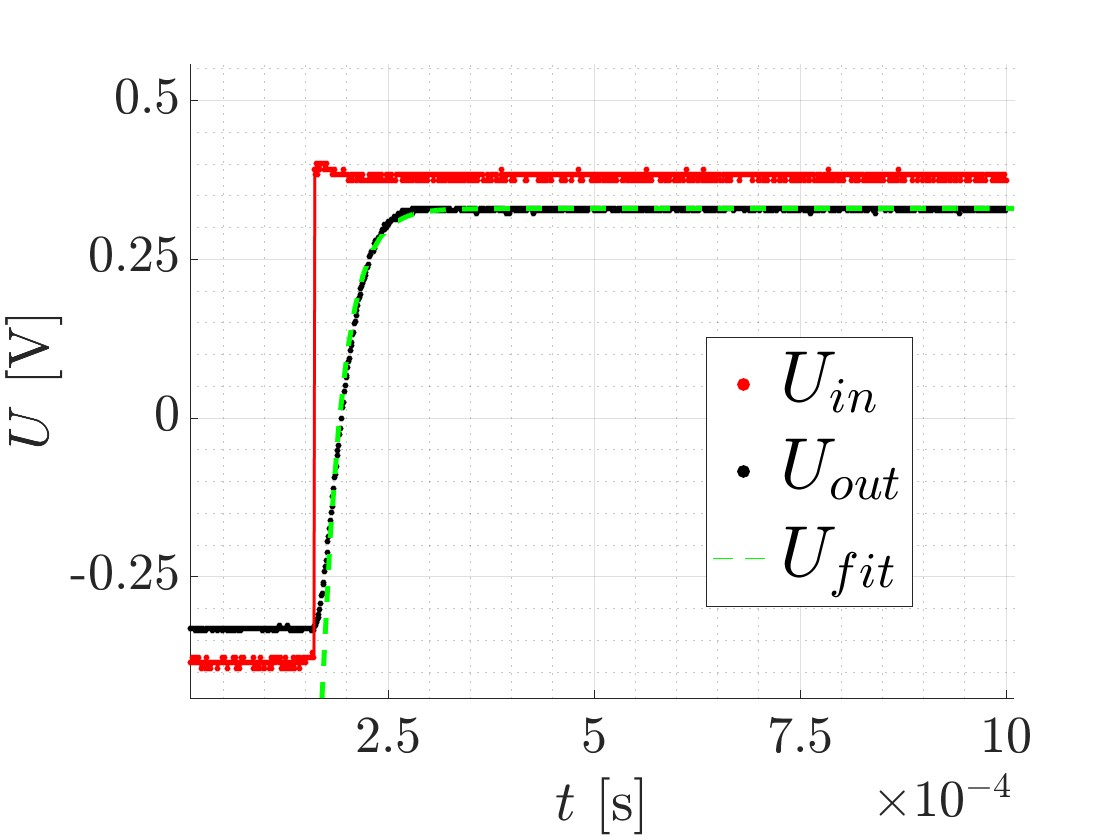
\includegraphics[width=1.2\linewidth,height = 6cm]{Graphes/critique/critique}
\vspace{-0.7cm}
\captionsetup{justification=centering}
\caption{Régime critique\\
$R = 1240\,\Omega$ et $\lambda_{exp} = (9 \pm 1)$ ms$^{-1}$}
\label{fig3}
\vspace{-0.7cm}
\end{wrapfigure}
\vspace{-0.2cm}
\begin{wrapfigure}{h}{0.5\textwidth}
\vspace{-1.7cm}
\raggedleft  % Pour centrer la figure
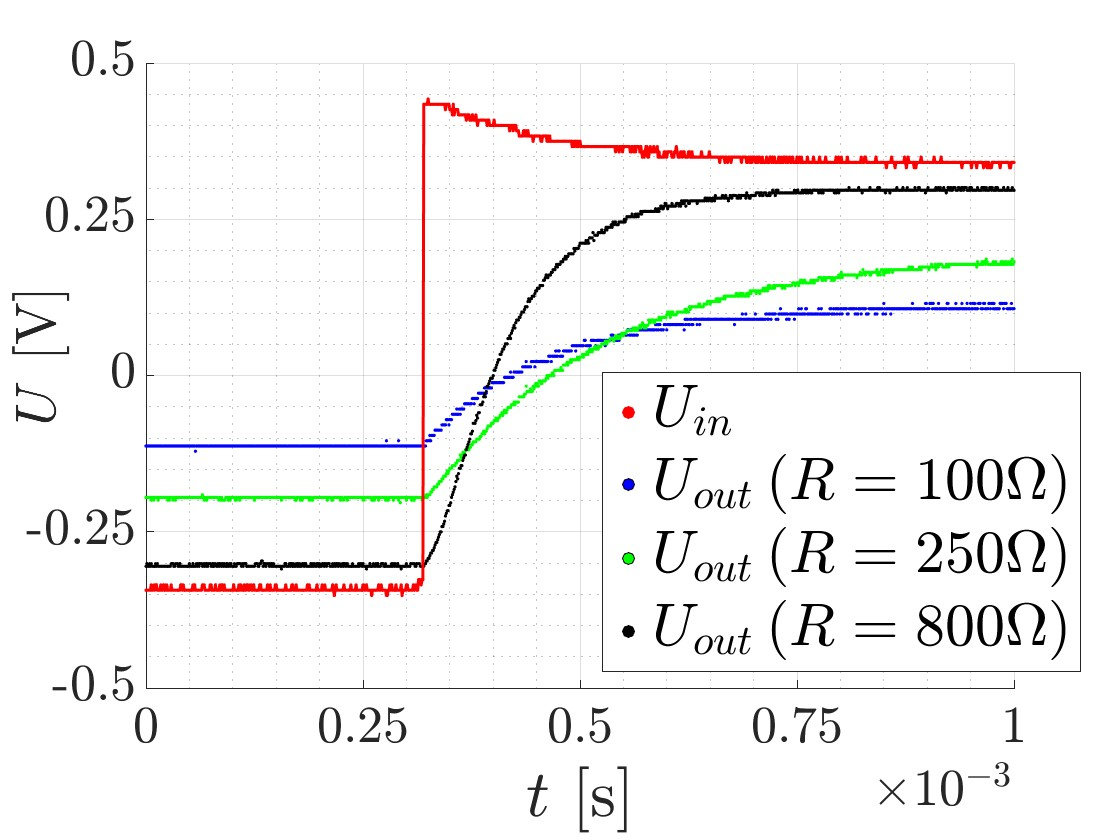
\includegraphics[width=1\linewidth, height=6cm]{Graphes/surcritique/surcritique.jpg}
\captionsetup{justification=raggedright}
%\caption{$R =(10\pm 0.1)$ k$\Omega$}
\vspace{-0.7cm}
\captionsetup{justification=centering}
\caption{Régime surcritique pour les résistances $R = 100\,\Omega,\,250\,\Omega$ et $800\,\Omega$}
\label{fig4}
\vspace{-1cm}
\end{wrapfigure}
\vspace{-0.2cm}
\begin{table}[b]
\centering
 \begin{tabular}{||c| c| c| c| c| c||} 
 \hline
 $R$ [k$\Omega$] & $\lambda$ [ms$^{-1}$] & $\lambda_{th}$ [s$^{-1}$] & $\lambda_{th,corr}$ [ms$^{-1}$] & $\epsilon_{th}$ [\%] & $\epsilon_{corr}$ [\%]\\ [0.5ex] 
 \hline\hline
% $1.024\pm 0.010$ & $40\pm 5$ & $49000\pm 2900$ & $51500\pm 2900$ & $18$ & $22$ \\ 
 %\hline
 $10 \pm 0.1$ & $7.8 \pm 1.3$ & $5000 \pm 300$ & $7570 \pm 300$ & $56$ & $3$\\
 \hline
 $50 \pm 0.5$ & $3.3 \pm 0.4$ & $1000\pm 60$ & $3570\pm 60$ & $230$ & $7$ \\
 \hline
 $900 \pm 9$ & $2.6 \pm 0.3$ & $55 \pm 3 $ & $2625 \pm 7$ & $460$ & $0$\\
\hline
\end{tabular}
\captionsetup{justification=centering}
\caption{Valeurs de $\lambda_{exp}$ comparées aux valeurs théoriques, avec calcul de l'erreur en régime sous-critique}
\label{table1}
\vspace{-0.5cm}
\end{table}
\clearpage

\subsection*{Oscillations forcées}

Dans le cas des oscillations forcées, la valeur de la résistance interne du circuit varie. En effet, $R_{in}=R_L=(207.0\pm 0.3)\,\Omega$. Le générateur de fonction maintient une tension $U_{in}$ à haute fréquence avec une amplitude maximale de $0.5$ V pour analyser le gain et la phase du signal. Les mesures sont effectuées à partir des paramètres suivants: les fréquence allant de $2$ kHz à $30$ kHz avec des incréments de 200 par décade. Les valeurs des résistances du circuit mesuré sont $10$ k$\Omega$, $50$ k$\Omega$ et $900$ k$\Omega$. La pulsation harmonique du système vaut ici $w_0 = (7100 \pm 200)$ Hz. Pour chaque valeur de la résistance, les valeurs de $\Omega_r,\,\Delta\Omega,\,Q,\,$et$\lambda_{exp}$ ont été mesurées à partir des graphes sur Fig.(\ref{fig5a}), Fig.(\ref{fig5b}) et calculées et comparées aux valeurs théoriques dans le tableau (\ref{table2}). $\lambda_{exp}$ sera calculé à l'aide de l'équation (\ref{eq_lambda}).
Dans les calculs de $\Omega_{th}$, une conversion s'effectue de rad.s$^{-1}$ en Hz par un facteur 2$\pi$, pour comparer les valeurs expérimentales et théoriques de la fréquence de résonance.

\begin{figure}[h]
\centering  % Centrer tout l'ensemble
\begin{subfigure}{0.49\textwidth}  % Réduire la taille pour s'assurer qu'elles tiennent côte à côte
    \centering  % Centrer cette sous-figure
    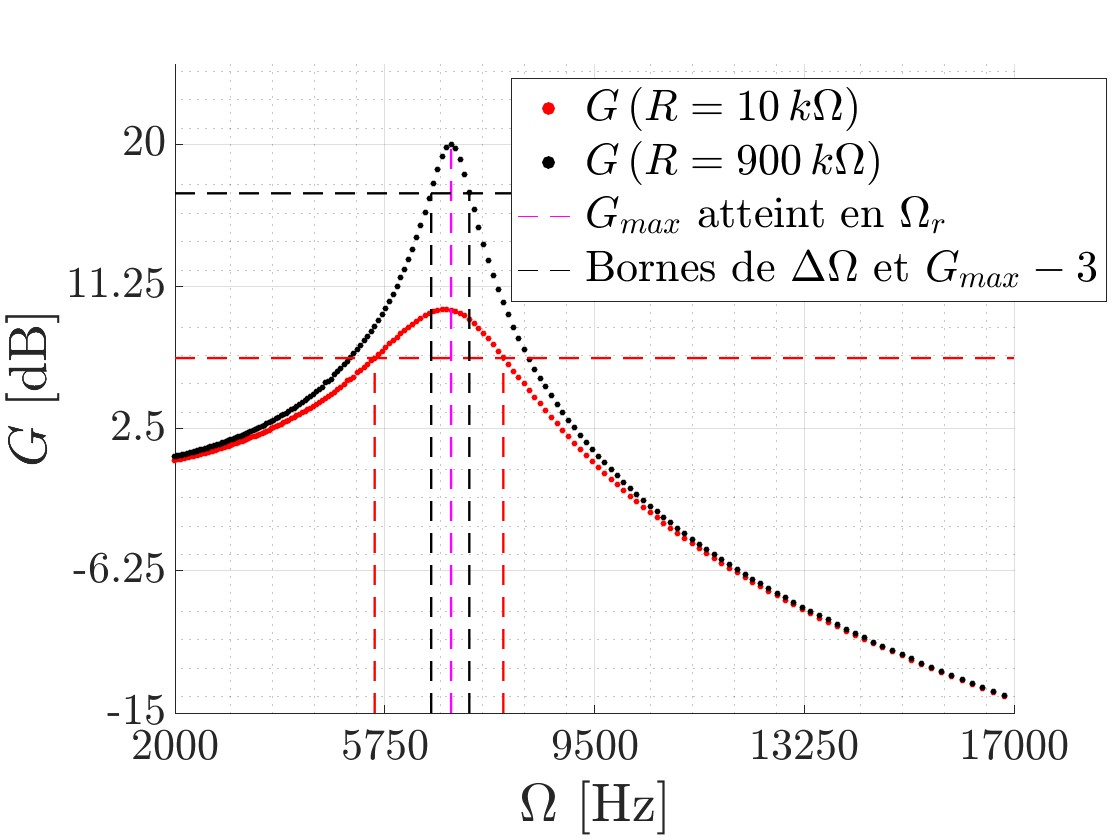
\includegraphics[width=1\linewidth, height=6cm]{Graphes/Gain/Gain}
    \captionsetup{justification=centering}
    \caption{$R =(10\pm 0.1)$ k$\Omega,\,\lambda_{exp} = (6.5 \pm 2)$ ms$^{-1}$}
    \label{fig5a}
\end{subfigure}
\begin{subfigure}{0.49\textwidth}  % Réduire également ici
    \centering  % Centrer cette sous-figure
    \includegraphics[width=1\linewidth, height = 6cm]{Graphes/Phase/phase}
    \captionsetup{justification=centering}
    \caption{$R =(50\pm 0.5)$ k$\Omega,\,\lambda_{exp} = (2.8 \pm 0.4)$ ms$^{-1}$}
    \label{fig5b}
\end{subfigure}
\captionsetup{justification=centering}
\caption{Diagramme de Bode du gain $G$ [dB] et graphe de la phase $\phi$ [deg] en fonction de $\Omega$ [Hz] pour deux valeurs de $R = 10$ k$\Omega$ et $R = 900$ k$\Omega$ en régime souscritique}
\label{fig5}
\end{figure}

\begin{table}[h]
\centering
 \begin{tabular}{||c| c| c| c| c| c| c| c| c|c ||}
 \hline
 $R$ [k$\Omega$] & $\lambda_{exp}$ [ms$^{-1}$] & $\Omega_{r}$ [Hz]& $\lambda_{th corr}$ [s$^{-1}$] & $\Omega_{r_{th}}$ [Hz]&$\epsilon_{\lambda_{corr}}$ [\%]  & $\epsilon_{\Omega_r}$ [\%]\\ [0.5ex] 
 \hline\hline
 $10 \pm 0.1$ & $7155 \pm 30$ & $6777 \pm 20$ & $7070 \pm 300$ & $6910\pm 200$ & $1$ & $2$  \\
 \hline
 $50 \pm 0.5$ & $3146 \pm 2$ & $6935\pm 3$ & $3070\pm 60$ & $7072 \pm 200$ & $2$ & $2$ \\
 \hline
 $900 \pm 9$ & $2191 \pm 4$ & $6935\pm 3$ & $2125 \pm 7$ & $7093 \pm 200$ & $3$ & $2$\\
\hline
\end{tabular}
\captionsetup{justification=centering}
\caption{Valeurs de $\lambda_{exp}$ et $\Omega_r$ comparées aux valeurs théoriques, avec calcul de l'erreur}
\label{table2}
\vspace{-0.2cm}
\end{table}

\begin{wraptable}{h}{0.4\textwidth}
\vspace{-0.3cm}
\raggedleft
 \begin{tabular}{||c| c|c||} 
 \hline
 $R$ [k$\Omega$] &$\Delta\Omega$ [Hz] & $Q$\\ [0.5ex] 
 \hline\hline
 $10 \pm 0.1$ & $2300\pm 4$ & $2.9\pm 0.8$ \\ 
 \hline
 $50 \pm 0.5$ & $1002 \pm 6$ & $6.9 \pm 0.3$ \\
 \hline
 $900 \pm 9$ & $682 \pm 5$ & $10.2\pm 0.4$\\
\hline
\end{tabular}
\captionsetup{justification=raggedleft}
\caption{Valeurs de $\Delta\Omega$ et $Q$}
\label{table3}
%\vspace{-0.5cm}
\end{wraptable}


Enfin, la dernière mesure du circuit repose sur l'inversemement de la capacité $C$ et de l'inductance $L$ dans le montage avec l'usage d'une résistance de \\$10$ k$\Omega$. La comparaison du montage original avec le montage inversé se trouve sur les Fig.(\ref{fig6a}) et Fig.(\ref{fig6b}). Les valeurs du gain et de toutes les autres caractéristiques du circuit inversé: $\Omega_r,\,\Delta\Omega,\,Q,\,$ et $\lambda_{exp}$ sont égales à celles de l'original.

\begin{figure}[t]
 % Centrer tout l'ensemble
\begin{subfigure}{0.49\textwidth}  % Réduire la taille pour s'assurer qu'elles tiennent côte à côte
    \centering  % Centrer cette sous-figure
    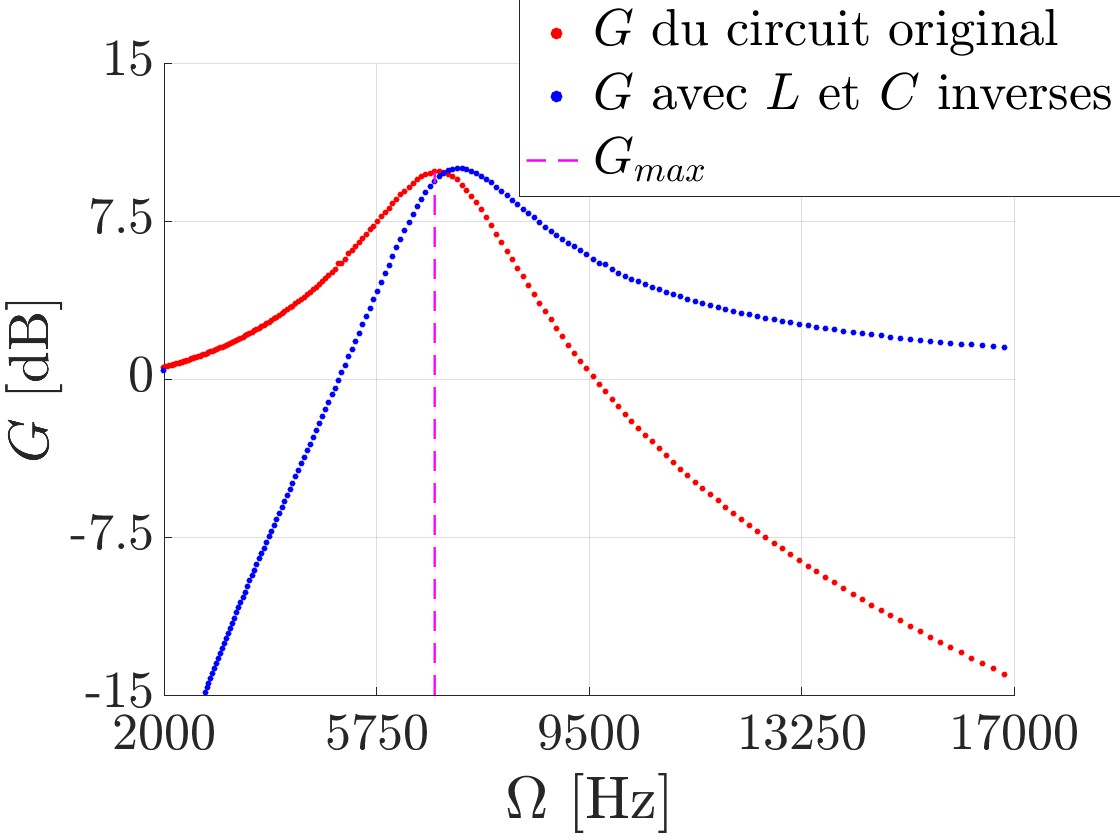
\includegraphics[width=1\linewidth, height=6cm]{Graphes/comparaison/Gain_compare}
    \caption{}
    \label{fig6a}
\end{subfigure}
\begin{subfigure}{0.49\textwidth}  % Réduire également ici
    \centering  % Centrer cette sous-figure
    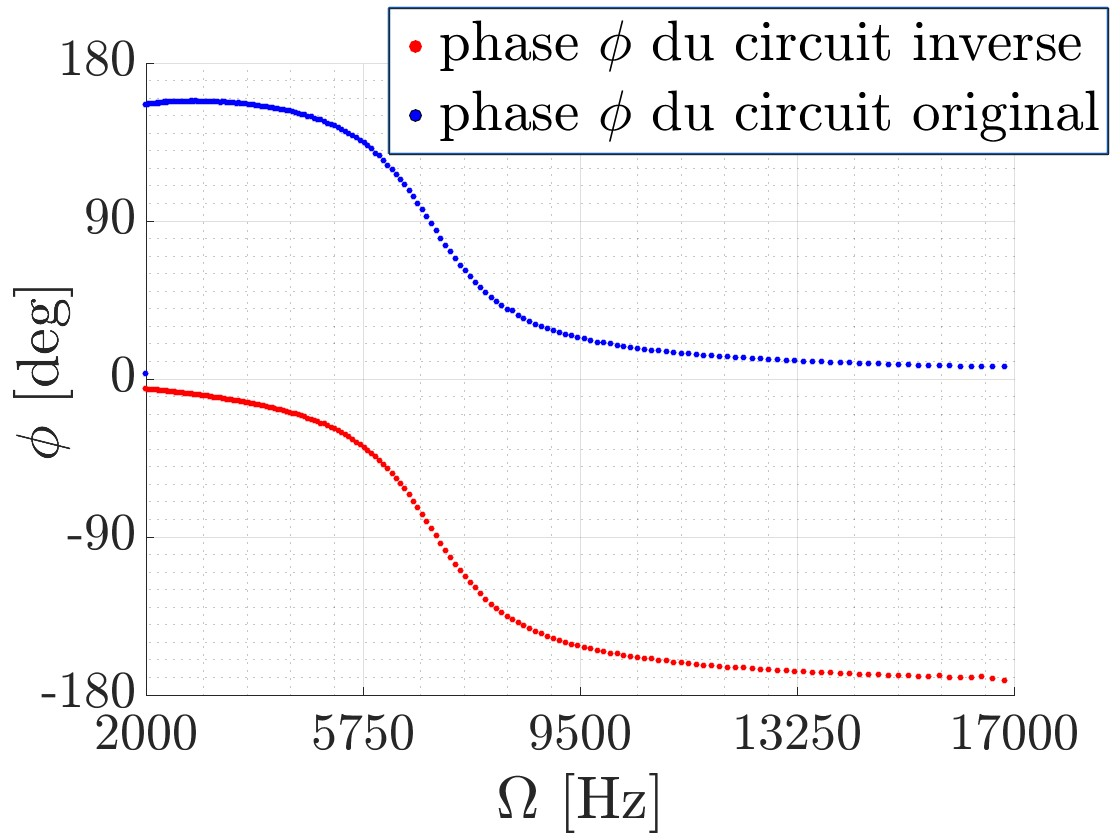
\includegraphics[width=1\linewidth, height = 6cm]{Graphes/comparaison/phase_comparer}
    \caption{}
    \label{fig6b}
\end{subfigure}
\captionsetup{justification=centering}
\caption{Diagramme de Bode du gain $G$ [dB] et graphe de la phase $\phi$ [deg] en fonction de $\Omega$[Hz] avec $R = 10$ k$\Omega$  en régime du circuit original et de celui avec $L$ et $C$ echangés}
\label{fig6}
\vspace{-0.5cm}
\end{figure}
\vspace{-0.8cm}

\section{Discussion}
\vspace{-0.3cm}

\subsection*{Oscillations libres}

Malgré un signal d'entrée d'amplitude non nulle, la forme carrée et la très faible fréquence $f$ du signal permettent de simuler une légère impulsion appliquée au système avant son retour au repos. Il s'agit du phénomène recherché pour les oscillations libres. En régime sous-critique, les Fig.(\ref{fig2a}) et Fig.(\ref{fig2b}) présentent la diminution de la résistance du système (toujours plus élevée que la résistance critique) entraînant la diminution de l'amplitude du signal de sortie avant son retour à une position d'équilibre. Comme le suggère l'expression même du coefficient d'amortissement, la baisse de la résistance provoque l'augmentation de $\lambda$, et donc de la pulsation $w$ du signal qui diminue jusqu'à ne plus osciller.\\
Quant au coefficient $\lambda$, sa mesure est effectuée à l'aide d'un fit exponentiel sur l'enveloppe de l'oscillation. La forte imprécision de la valeur $\lambda_{exp}$ mesurée s'explique ainsi par les incertitudes de mesures, du fit mais aussi le faible nombre de données utilisées pour la production du fit. Pour améliorer ce point, augmenter la fréquence d'échantillonnage ou moyenner les mesures de $\lambda_{exp}$ pour la même résistance sont des solutions optimales.\\
Dans le tableau (\ref{table1}), la croissance de $R$ à partir de $R_{cr}$ implique une décroissance de $\lambda$ qui ne semble absolument pas correspondre à la valeur théorique $\lambda_{exp}$. En effet, la croissance de l'erreur relative $\epsilon_{th}$ de $\lambda_{exp}$ (56\%, 230\%, 460\%) avec l'augmentation de $R$ démontre l'importance de la prise en compte de la résistance interne des composantes du circuit pour déterminer $\lambda_{exp}$. Le terme constant dans l'equation (\ref{eq'}) $R_{in}/(2L)$ induit un décalage de 2570 Hz entre la valeur $\lambda_{th}$ purement théorique et $\lambda_{th,corr}$. Cette différence devient fondamentale dès que la résistance $R$ du circuit n'est plus de l'ordre de $R_{rc}$. Après considération, $\lambda_{th,corr}$ est très proche de $\lambda_{exp}$, l'erreur résultant est ainsi de l'ordre de 5 \%, résultat satisfaisant les attentes de la théorie. La non-nullité (3\%,7\%) de cette erreur relative s'explique sûrement par les incertitudes de mesure, de fits ainsi que par la résistance interne des autres composantes du circuit comme les fils.\\
Pour le régime critique, le comportement du système est bien celui attendu sur la Fig.(\ref{fig3}). Lorsque $R = R_{rc}$ la tension $U_{out}$ converge au plus vite vers la tension d'entrée $U_{in}$. Par ailleurs, la valeur mesurée $\lambda_{exp} = (9 \pm 1)$ ms$^{-1}$ dans ce régime est tout à fait cohérente avec la valeur attendue étant donné que $w_0 = (7100 \pm 200)$ Hz et qu'il faut toujours tenir compte des résistances internes. De plus, le fit effectué sur ce régime est moins précis que le précédent par manque de mesures, donc l'erreur admise est cohérente.\\
Enfin, le régime surcritique, présenté sur la Fig.(\ref{fig4}), montre un retour sans oscillation vers la position d'équilibre. La tendance du système à revenir à l'équilibre est bien corrélé au coeffcient d'amortissement et donc de la résistance utilisée dans le montage. Cet amortissement s'avère suffisament puissant selon la résistance pour ne pas laisser le système revenir à l'équilibre avant la prochaine impulsion du signal d'entrée.
Les comportements observés sur ces trois régimes correspondent bien à ceux décrits par la théorie en particulier à l'équation (\ref{eq_boss}).
\vspace{-0.4cm}
\subsection*{Oscillations forcées}

Dans ce type d'oscillation, le système se caractérise par son comportement lorsqu'il entre en résonance. La Fig.(\ref{fig5a}) montre qu'avec l'utilisation toujours plus grande de résistance $R > R_{rc}$, le gain maximal $G_{max}$ atteint en résonance croît alors que la fréquence $\Omega_r$ diminue, cette réaction s'explique par la diminution de $\lambda_{exp}$ conforme à la théorie. Il en va de même pour le facteur de qualité de la résonance $Q$ puisque la finesse de la résonance diminue($\Delta\Omega$ décroît). Un cas particulier est la nullité du coefficient d'amortissement $\lambda$, possible lorsque ($RC\rightarrow\infty$), qui conduit à un gain $G_{max} = \infty$ lorsque le système entre en résonnace. Un léger déphasage entre $w_0$ et $\Omega_r$ se remarque lorsque la résistance utilisée est de l'ordre de $R_{rc}$, ce qui est cohérent avec l'expression de la fréquence de pulsation. Dans le tableau (\ref{table2}), l'erreur relative $\epsilon_{\Omega_r}$ reste constante (2 \%) mais compte tenu du faible nombre de mesures, la valeur théorique ne peut pas être considérée comme très fiable, notamment car la valeur de $\Omega_r$ ne varie pas expérimentalement pour $R = 50$ k$\Omega$ et $R=900$ k$\Omega$ ($\Omega_r = 6935$ Hz), tandis que la valeur théorique change $\Omega_{r_{th}}: 7072 \text{Hz}\,\rightarrow 7093$ Hz, malgré l'incertitude de ces deux valeurs. D'un autre côté, la valeur $\lambda_{exp}$ dans le tableau(\ref{table2}) calculée à partir de l'équation (\ref{eq_lambda}) est restée similaire à celle calculée à l'aide des fits, compte tenu des incertitudes. Cette constance affirme la précision du résultat. De plus, la valeur théorique attendue $\lambda_{th,corr}$ a varié, entraîné par la variation de la résistance interne du circuit ($R_G$ pris en compte par le logiciel). Par conséquent, l'erreur relative $\epsilon_{th}$ de $\lambda_{th,corr}$ du tableau (\ref{table2}) de l'ordre de 4 \% a diminué par rapport à celle du tableau (\ref{table1}) avec des erreurs de l'ordre de 2 \%. En plus, d'une erreur plus faible, cette technique offre une incertitude bien plus faible passant d'un ordre de 500 Hz sur le tableau (\ref{table1}) à une incertitude bien plus précise de l'ordre de 10 Hz sur le tableau (\ref{table2}). Faut-il en conclure que la deuxième méthode est plus convenable? Cette conclusion est très probable mais pas certaine à cause du manque de mesures effectuées. La dernière expérience était l'inversion des dipôles $L$ et $C$ qui provoque un comportement symétrique à celui du circuit original sur la figure Fig.(\ref{fig6a}). En effet, cette pseudo-symétrie se produit autour de la fréquence de résonance $\Omega_r$. Alors que le circuit original, amplifiait légèrement, le signal dans les faibles fréquences et atténuait fortement les hautes fréquences, le circuit inversé atténue les faibles fréquences et amplifie les hautes fréquences. Il s'agit du comportement d'un filtre passe-haut pour le circuit original et d'un filtre passe-bas pour le circuit inversé. Une approximation de la pente de ces filtres dans leur phase d'atténuation est d'environ 20 dB par décade, ce sont des filtres du deuxième ordre. La fréquence de résonance $\Omega_r$ de ces deux circuits est égale et la phase est de 90° mais négative pour le circuit original et positive pour celui inversé.
\vspace{-0.5cm}
\section{Conclusion}
Tous les modes d'oscillations ont été étudiés et ont permis de mettre en évidence les caractéristiques du circuit RCL. Dans chaque cas de figure, des mesures ont été effectuées pour estimer les erreurs des valeurs théoriques du circuit. L'ensemble des résultats ont été conformes à ceux attendus par la théorie. La considération de certains facteurs propre au montage utilisé ont été fondamental pour ces estimations, en particulier la précision des appareils de mesures utilisés et les résistances internes du circuit. Des propriétes cruciales des filtres passe-haut et passe-bas ont été présentées. Ainsi, les comportements oscillatoires ci-observés permettent de mieux comprendre la mécanique oscillatoire et donc répondre à de nouveaux problèmes.

\section{Références}
% Redéfinir le format des numéros dans l'environnement enumerate
\renewcommand{\labelenumi}{[\theenumi]}
\begin{enumerate}
    \item \label{ref1} SKYbrary, Oscillation induite par le pilote:\\\url{https://skybrary.aero/articles/pilot-induced-oscillation}
    \item \label{Tacoma} Wikipedia, Pont du détroit de Tacoma (1940): \\\url{https://fr.wikipedia.org/wiki/Pont_du_détroit_de_Tacoma_(1940)}
    \item \label{ref9} EPFL, TP Physique, Traitement des erreurs de mesure, Moodle:\\ \url{https://moodle.epfl.ch/pluginfile.php/3003789/mod_resource/content/2/Erreurs_2022.pdf}
    \item \label{ref0} EPFL, TP2 expériences notices, G3. RLC Circuits: \\\url{https://www.epfl.ch/schools/sb/sph/wp-content/uploads/G3_RLC_Circuits.pdf}
\end{enumerate}

\section{Incertitudes}
Le multimètre possède une incertitude de $\pm 3$ sur le dernier digit. Cette incertitude a été prise en compte dans la mesure de $R_L$.
D'après les informations données par le fabriquant, les machines employées ont pour incertitudes:
\[
    \frac{\Delta L}{L} = 0.05 \qquad
    \frac{\Delta R}{R} = 0.01 \qquad
    \frac{\Delta C}{C} = 0.01 \qquad
\]

De plus, par le calcul, les expressions suivantes sont les incertitudes des valeurs mesurées, l'ensemble des valeurs étant positives, l'inutilisation de valeurs absolues allège les expressions:
\[
    \Delta \lambda_{th} = \lambda_{th} \left( \frac{\Delta C}{C} + \frac{\Delta R}{R} \right)
\]

\[
    \Delta \lambda_{th, \text{ corr.}} = \Delta \lambda_{th} + \frac{1}{2L} \left( \frac{\Delta L}{L} + \frac{\Delta R_{in}}{L} \right)
\]

\[
    \Delta \omega_0 = \frac{1}{2} \omega_0 \left( \frac{\Delta L}{L} + \frac{\Delta C}{C} \right)
\]

\[
    \Delta \omega = \frac{\omega_0 \Delta \omega_0 + \lambda \Delta \lambda}{\omega}
\]

\[
    \Delta \Omega_r = \frac{\omega \Delta \omega + 2 \lambda \Delta \lambda}{\Omega_r}
\]
Pour l'équation (\ref{eq_lambda}), l'incertitude du calcul est la suivante:
\[
    \Delta\lambda_{exp} = \Delta\Omega_{r_{exp}}\sqrt{\frac{1}{2}\left(\sqrt{\frac{G_{max}^2}{G_{max}^2-1}}-1\right)}+\left| \frac{-\Omega_{r_{exp}}G_{max}\Delta G_{max}}{8\sqrt{\frac{1}{2}\left(\sqrt{\frac{G_{max}^2}{G_{max}^2-1}}-1\right)}\sqrt{\frac{G_{max}^2}{G_{max}^2-1}}(G_{max}^2-1)^2} \right|
\]
Les incertitudes des valeurs expérimentales, lues sur les graphiques à l'aide du curseur, ont été choisies pour couvrir largement la valeur attendue.


\end{document}